\documentclass[tikz,border=10pt]{standalone}
\begin{document}
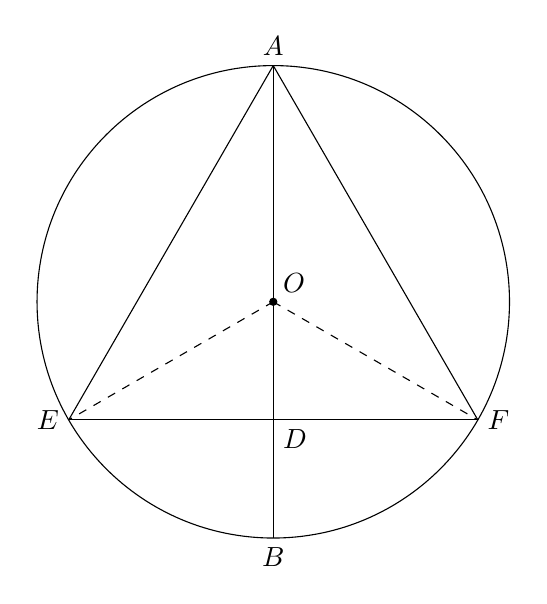
\begin{tikzpicture}
    % Define coordinates
    % Let radius be 3cm.
    % Center O at (0,0)
    \coordinate (O) at (0,0);
    
    % A is top, B is bottom
    \coordinate (A) at (0,3);
    \coordinate (B) at (0,-3);
    
    % Chord EF is horizontal below the center.
    % Let's place D at (0, -1.5).
    \coordinate (D) at (0,-1.5);
    
    % E and F are on the circle x^2 + y^2 = 9.
    % y = -1.5 => x^2 + 2.25 = 9 => x^2 = 6.75 => x = sqrt(6.75) approx 2.598
    \coordinate (E) at (-2.598, -1.5);
    \coordinate (F) at (2.598, -1.5);

    % Draw the circle
    \draw (O) circle (3);

    % Draw solid lines
    \draw (A) -- (B);       % Vertical diameter
    \draw (E) -- (F);       % Horizontal chord
    \draw (A) -- (E);       // Chord AE
    \draw (A) -- (F);       // Chord AF

    % Draw dashed lines
    \draw[dashed] (O) -- (E);
    \draw[dashed] (O) -- (F);

    % Mark center O with a dot
    \fill (O) circle (1.5pt);

    % Labels
    \node[above] at (A) {$A$};
    \node[below] at (B) {$B$};
    \node[left] at (E) {$E$};
    \node[right] at (F) {$F$};
    \node[above right] at (O) {$O$};
    \node[below right] at (D) {$D$};
\end{tikzpicture}
\end{document}
